\documentclass[11pt]{article}

\usepackage[margin=1in]{geometry}
\usepackage{amsmath, amssymb}
\usepackage{booktabs}
\usepackage{xcolor}
\usepackage{enumitem}
\usepackage{hyperref}
\usepackage{float}
\usepackage{graphicx}

\definecolor{notecol}{rgb}{0.15,0.35,0.6}
\definecolor{todocol}{rgb}{0.7,0.3,0.0}

% One decision / measurement per entry, appended at the end in date order:
%   \entry{ID. Title}{YYYY-MM-DD}{anchor}{Topic}
% IDs: D decision, M measurement, O open, T tooling. Fields in the order listed below.
% A new date starts a new day heading; \topicindex lists the entries by topic.
\makeatletter
\newcommand{\nb@lastdate}{}
\def\nb@topics{}
\newcommand{\entry}[4]{%
  \def\nb@date{#2}%
  \ifx\nb@date\nb@lastdate\else
    \section*{#2}\addcontentsline{toc}{section}{#2}%
    \global\let\nb@lastdate\nb@date
  \fi
  \subsection*{#1 \hfill \small\normalfont\textsc{#4}}%
  \addcontentsline{toc}{subsection}{#1}\label{#3}%
  \nb@addtopic{#4}{#1}{#3}}
\newcommand{\nb@addtopic}[3]{%
  \@ifundefined{nb@topic@#1}{%
    \expandafter\gdef\csname nb@topic@#1\endcsname{}%
    \g@addto@macro\nb@topics{\nb@printtopic{#1}}}{}%
  \expandafter\g@addto@macro\csname nb@topic@#1\endcsname{\item \hyperref[#3]{#2}}}
\newcommand{\nb@printtopic}[1]{\item[#1]%
  \begin{itemize}[nosep]\csname nb@topic@#1\endcsname\end{itemize}}
\newcommand{\topicindex}{\ifx\nb@topics\@empty\else
  \section*{Entries by topic}\addcontentsline{toc}{section}{Entries by topic}%
  \begin{description}[style=nextline]\nb@topics\end{description}\fi}
\makeatother
\newcommand{\field}[1]{\par\smallskip\noindent\textbf{#1.}\ }
\newcommand{\verify}[1]{\textcolor{todocol}{[to verify: #1]}}
\newcommand{\file}[1]{\texttt{\detokenize{#1}}}

\title{Lab Notebook: SRAM Compute-in-Memory Macro in ASAP7}
\author{Daniel Vigna}
\date{Started 2026-10-14}

\begin{document}
\maketitle

\section*{How this notebook works}
Every design decision and every measurement gets one entry, written when it happens and appended in date order. Each day starts a new heading, and every entry names the topic it touches (see \emph{Entries by topic} at the end). The fields of an entry:
\begin{description}[leftmargin=2em, style=nextline]
  \item[Question] what was being decided or measured.
  \item[Options] the alternatives considered.
  \item[Method] tool, testbench, corner, and the script or file that reproduces it.
  \item[Result] the numbers.
  \item[Decision] what was chosen and why.
  \item[Revisit if] the condition that would reopen it.
\end{description}
Claims that are reasoning but not yet measured are marked \verify{like this}.
Scripts live in \file{scripts/}, raw data in \file{data/}, next to this file (\file{~/papers/notebook/sram-cim} on the VM).

\paragraph{Setup (all entries unless noted).}
ASAP7 predictive 7\,nm PDK; OpenLayout flow (xschem, KLayout, FasterCap PEX, ngspice with BSIM-CMG);
SRAM-Vt devices (\file{nmos_sram}, \file{pmos_sram}) in the bitcell; TT models (\file{7nm_TT.pm}), $V_{DD} = 0.7$\,V.
Gate pitch (CPP) 54\,nm, cell height 270\,nm (one 7.5-track standard-cell row).

\tableofcontents

% =====================================================================
\entry{D3. 2-bit cell placement (b2SRAMsbc), 14 CPP}{2026-10-12}{d3}{Bitcell}
\field{Question} Smallest placement of the 20-device 2-bit CIM cell (two 6T latches, two NOR2).
\field{Options} Original N/P/N frame, 16 CPP $\times$ 405\,nm; N/P frame at 270\,nm height.
\field{Method} Euler-path chaining: 6 odd-degree P nets $\Rightarrow$ at least 3 P chains $\Rightarrow$ 14 CPP minimum; every P gate column shares poly with an N gate of the same net. Unchained transistors keep LISD two gate pitches apart (double diffusion break). KLayout DRC.
\field{Result} 14 CPP $\times$ 270\,nm, $-42\%$ area vs.\ the original, DRC clean; later routed to M3, DRC clean, LVS match. $0.756 \times 0.27\,\mu\text{m} = 0.204\,\mu\text{m}^2$, i.e.\ $0.102\,\mu\text{m}^2$ per bit.
\field{Decision} Kept as the dense reference point (superseded for now by D4).

\entry{D1. Dataflow: weight-stationary, bit-serial input}{2026-10-14}{d1}{Architecture}
\field{Question} How does an array of 1-bit AND cells compute a multiply?
\field{Options} (a) 8 parallel input bits per row (bitwise AND only); (b) one input bit per row per cycle, broadcast to all weight bits (bit-serial).
\field{Method} Reasoning; worked example below.
\field{Result} Each cell computes $P = \overline{\overline{Q} + \overline{X}} = Q \cdot X$. With (a) a row yields $W_i X_i$ for matching bits only, which is not a product. With (b) a row holding weight $W$ yields the partial product $W \cdot x[t]$ each cycle, and
\[ W \times X = \sum_{t=0}^{7} 2^t\,(W \cdot x[t]), \qquad \text{MSB first: } \mathrm{Acc} \leftarrow 2\,\mathrm{Acc} + P. \]
Example (4 bit): $W = 1101_2 = 13$, $X = 0110_2 = 6$: Acc $= 0, 13, 39, 78 = 13 \times 6$.
With several rows, the $P$ bits of each column are summed first (popcount), giving $\sum_i W_i\,x_i[t]$ per cycle; the same accumulator then forms the dot product $\sum_i W_i X_i$.
\field{Decision} (b). The weight stays in the SRAM and the input streams past it; a row is one reused row of AND gates of an array multiplier.
\field{Revisit if} throughput needs more than one input bit per cycle (e.g. 2-bit-serial inputs).

\entry{D2. Start with one 8$\times$1 row, not a full array}{2026-10-14}{d2}{Architecture}
\field{Question} What is the first block to build and verify?
\field{Options} (a) the full multi-row array with column adders; (b) a single row of 8 cells plus a shift-accumulate adder (an $8\times8$ bit-serial multiplier).
\field{Decision} (b). It exercises the cell, the NOR and the accumulator with nothing to add across rows; more rows later only insert per-column adders between the row and the accumulator.
\field{Revisit if} n/a (staging decision).

\entry{D4. 1-bit 10T cell instead of the 2-bit cell}{2026-10-14}{d4}{Bitcell}
\field{Question} Use the dense 2-bit cell, or a simpler 1-bit cell (6T + one NOR2)?
\field{Options} (a) b2SRAMsbc: two latches share BL/BL\_Bar, selected by WL[1]/WL[0]; (b) SRAMCIMsbc: one latch, one NOR.
\field{Method} Layout in OpenLayout; DRC and LVS (\file{data/cells/}); bounding box via \file{scripts/bbox.rb}.
\field{Result} SRAMCIMsbc: 10 CPP $\times$ 270\,nm $= 0.146\,\mu\text{m}^2$ per bit, DRC clean, LVS match. That is $+43\%$ area per bit vs.\ (a).
\field{Decision} (b). The 2-bit array's mapping (two weights interleaved per cell row, shared bitlines) made the design hard to reason about; the 1-bit cell keeps one cell = one weight bit while the dataflow is being learned.
\field{Revisit if} area becomes the main metric, or once the 1-bit design works end to end (the 2-bit cell is "two 1-bit cells stacked", so the architecture carries over).

\entry{D5. NOR2 sizing}{2026-10-14}{d5}{Bitcell}
\field{Question} Fin counts of the NOR's series pMOS and parallel nMOS.
\field{Options} p1/n2 (as in b2SRAMsbc); 2/2; p2/n1.
\field{Method} RC reasoning relative to a 1-fin inverter, assuming similar drive per fin for n and p in ASAP7 \verify{per-fin $I_{on}$ of nmos\_sram vs.\ pmos\_sram at TT}.
\field{Result} Pull-up of two series devices vs.\ worst-case pull-down of one device: p1/n2 $\Rightarrow$ rise $\approx 4\times$ slower than fall; 2/2 $\approx 2\times$; p2/n1 $\approx$ balanced. The slow edge is $P$ rising ($Q=1$, $X=1$), which sets the compute delay. Extra nMOS fins only add gate load on the storage node and on XB.
\field{Decision} p2/n1 in SRAMCIMsbc.
\field{Revisit if} the measured rise/fall from the PEX row testbench disagrees, or the N chain forces 2-fin nMOS.

\entry{D6. Latch sizing and read path}{2026-10-14}{d6}{Bitcell}
\field{Question} PU/PG/PD = 1/2/2 fins gives a cell ratio $\beta = 1$; is that safe?
\field{Result} A classic bitline read with $\beta = 1$ risks read disturb \verify{read SNM at TT}. The CIM cell does not need bitline reads: driving $X = 1$ shows the stored bit on $P$, and the NOR loads the storage node with gate capacitance only.
\field{Decision} Keep 1/2/2; read through the NOR, no sense amplifiers.
\field{Revisit if} a conventional SRAM read mode is wanted.

\entry{D7. XB driver: INVx1}{2026-10-14}{d7}{Row}
\field{Question} Which inverter drives the row's XB line?
\field{Options} INVxp67 (2+2 fins), INVx1 (3+3), INVx2 (6+6) from \file{asap7sc7p5t_28_R}.
\field{Method} Load per cell: NOR nMOS 1 fin + pMOS 2 fins = 3 fins; 8 cells = 24 fins, plus $\approx 0.17$\,fF of XB wiring per cell (PEX). Electrical fanout = load / input fins.
\field{Result} INVx1: FO $\approx 4$--5. INVx2: FO $\approx 2$--2.5 but doubles the load on the stage driving it. The inverter also produces XB from the true input bit, and the 270\,nm standard-cell height matches the bitcell, so it can abut the row.
\field{Decision} INVx1 \verify{XB edge and P delay with INVx1 vs.\ INVx2 on the 1$\times$8 PEX row}.
\field{Revisit if} XB fans out to more weights (an $8\times8$ matrix: 64 cells, $\approx$190 fins, FO $\approx 32$ for INVx1 $\Rightarrow$ two-stage buffer, e.g.\ INVx1 $\rightarrow$ INVx4).

\entry{O1. Row schematic status (SRAMCIMsbc\_INT8)}{2026-10-14}{o1}{Row}
WL and BL[7:0]/BLB[7:0] wired (x1 = bit 7). Open: XB tied to one net with an \file{ipin}; P labelled P[7:0] with an \file{opin}. Symbol: XB (left) and P (right) share $y = 10$, which shorts P$_k$ to XB$_{k+1}$ on abutment; plan: XB pass-through on both edges, P on the bottom edge, matched in layout.

\entry{M1. Flat PEX and SPICE scaling}{2026-10-14}{m1}{Verification}
\field{Question} How large an array can be extracted and simulated flat overnight ($\le 8$\,h)?
\field{Method} SRAMCIMsbc tiled $1\times8$ and $2\times8$ (\file{scripts/tile.py}: 0.54\,$\mu$m pitch, odd rows mirrored); \file{openlayout pex} (FasterCap 3D); 12\,ns ngspice transient (\file{scripts/tb_*.sp}). VM: 8 vCPU, 10\,GB RAM. Raw: \file{data/pex-scaling/}.
\field{Result}
\begin{table}[H]\centering\small
\begin{tabular}{lrrrrrr}
\toprule
Layout & Cells & Conductors & FasterCap (s) & Memory (GB) & Capacitors & ngspice (s) \\
\midrule
1 cell        & 1  & 16  & 3.3   & 0.46 & 222    & 0.85 \\
$1\times8$    & 8  & 107 & 322   & 0.50 & 3\,684  & 37.8 \\
$2\times8$    & 16 & 197 & 971   & 1.02 & 17\,662 & failed$^\dagger$ \\
\bottomrule
\end{tabular}

\smallskip
$^\dagger$ operating point failed; the tiles were not wired as a real array, so treat as order-of-magnitude.
\end{table}
FasterCap time grows roughly as $(\text{conductors})^{1.8\text{--}2.3}$; capacitor count roughly quadratically. Extrapolated: $\approx$1\,300 conductors ($\approx$100 cells) fit in 8\,h at $\approx$6--7\,GB; 640 weights $\times$ 8 bits ($\approx$5\,000 cells, $\approx$30\,000 conductors) would take months and $>$100\,GB.
\field{Decision} Never extract or simulate the full array flat. Verification ladder: (1) leaf-cell PEX, reused per instance; (2) critical paths with PEX: one row with full WL/XB load, one column with full BL load, the adder's slowest path; (3) function by a behavioral model (Python/Verilog) of the whole array on the full dataset.
\field{Revisit if} hierarchical PEX lands in OpenLayout (in progress), which changes the cost of step 2.

\entry{T1. OpenLayout/xschem fixes found while designing}{2026-10-14}{t1}{Tooling}
Symbol pins off the 10 grid (the symbol editor's 2.5 snap) could not be reached by schematic wires: pins now move on 10 when selected, and saving a symbol snaps strays (stubs kept straight, one undo). Copying several objects with \texttt{c} + a click on the selection kept only one: xschem's cadence-compat release trimmed the selection on command clicks. Fixed with xschem patches; OpenLayout commit \file{dc53d6b}.

\entry{D8. Back to the 2-bit cell: a 4-row array of 8 INT8 weights}{2026-10-16}{d8}{Architecture}
\field{Question} With the dataflow understood (D1), which cell and array shape does the signed INT8 design use?
\field{Options} (a) stay with the 1-bit 10T cell (D4); (b) the 2-bit cell b2SRAMsbc (D3), 8 cells per row, 4 rows.
\field{Method} Reasoning on the mapping, then the schematic \file{b2SRAMsbc_INT8x8.sch}, netlisted with xschem (32 cells; a script checked that every cell sits on the WL / XB / P / BL nets of its row and bit).
\field{Result} Each cell holds bit $j$ of two weights (latch 1 and latch 0, sharing BL/BLB). Row $r$ holds $W_{2r+1}$ (WL[$2r{+}1$], XB[$2r{+}1$], P$_{2r+1}$[7:0]) and $W_{2r}$ (WL[$2r$], XB[$2r$], P$_{2r}$[7:0]); 4 rows $\times$ 8 cells = 64 bits = 8 weights, BL[$j$]/BLB[$j$] shared down each column. Every NOR computes in the same cycle, so each bit column delivers 8 product bits per cycle: the column sum is an 8-input popcount (compressor tree), not a single add. The dot product $\sum_{i=0}^{7} W_i X_i$ of 8 signed $8\times8$ terms needs $8+8+3 = 19$ bits (worst case $8 \cdot (-128)(-128) = 2^{17}$). Area: $0.102\,\mu\text{m}^2$ per bit vs.\ $0.146$ for the 10T cell.
\field{Decision} (b). D4's reason (the 2-bit mapping was hard to reason about) no longer holds, and the 2-bit cell is 30\% smaller per bit.
\field{Revisit if} the shared bitlines complicate writes, or read disturb (D6) shows up in simulation.

\entry{D9. b2SRAMsbc NOR pMOS: 2 fins}{2026-10-16}{d9}{Bitcell}
\field{Question} Apply D5 to the 2-bit cell, whose NOR was p1/n2.
\field{Options} Widen the four NOR pMOS (M13, M14, M17, M18) to 2 fins in the existing 14-CPP placement, or re-place the cell.
\field{Method} Schematic nfin $1 \rightarrow 2$; in the layout only the PCell parameter \texttt{nfin} of those four instances (second fin on fin row 7, ACTIVE / LISD / SDT down to 189\,nm). Each widened device shares diffusion with a 1-fin latch pMOS, so the ACTIVE steps from 2 to 1 fin at the shared contact (DRC allows it). KLayout DRC, LVS, OpenLayout connectivity check.
\field{Result} LVS match. The wider LISD came 10\,nm from three LIG gate contacts (LIG--LISD/SDT spacing $\ge 14$\,nm, corner $\ge 15$): two were moved down 5\,nm; the third, wedged between the Q\_bar[1] LISD strap and the new LISD, was trimmed to $177$--$207 \times 144$--$174$\,nm, which keeps its LIG tip-to-side spacing at exactly 25\,nm. DRC clean, LVS match, no shorts or opens. Cell size unchanged (14 CPP $\times$ 270\,nm).
\field{Decision} 2/2 (p2/n2): the pull-up is no longer the $4\times$ slower edge \verify{P rise/fall on the PEX row}. The nMOS stay at 2 fins because the N row is one 2-fin chain.
\field{Revisit if} the P rise is still the slow edge after PEX.

\entry{D10. Array assembly: on the fin grid, bus pins}{2026-10-16}{d10}{Array}
\field{Question} How are the 32 cells placed and pinned?
\field{Method} Rows alternate unmirrored / mirrored about $x$ so neighbours share a rail (VSS at 270 and 810\,nm, VDD at 540\,nm); 14-CPP column pitch (756\,nm). DRC of the assembled layout. Symbol \file{b2SRAMsbc_INT8x8.sym}, checked by netlisting an instance (96 bus bits, instance and subcircuit in the same order).
\field{Result} The first placement put the rows at $y = 20, 290, \ldots$\,nm and every fin failed FIN.S.1: the fin grid is absolute (fin centrelines at $13.5 + 27k$\,nm from the layout origin), so a row origin must be a multiple of 27\,nm. Moving the array by $-20$\,nm cleared all 40 violations; every instance was already on the exact pitch. The symbol has 12 bus pins: BLB[7:0], BL[7:0] (top), WL[7:0], X[7:0] (left), P7[7:0] \ldots\ P0[7:0] (right); the schematic's per-bit BL/BLB/WL pins became labels plus bus pins so symbol and schematic match.
\begin{figure}[H]\centering
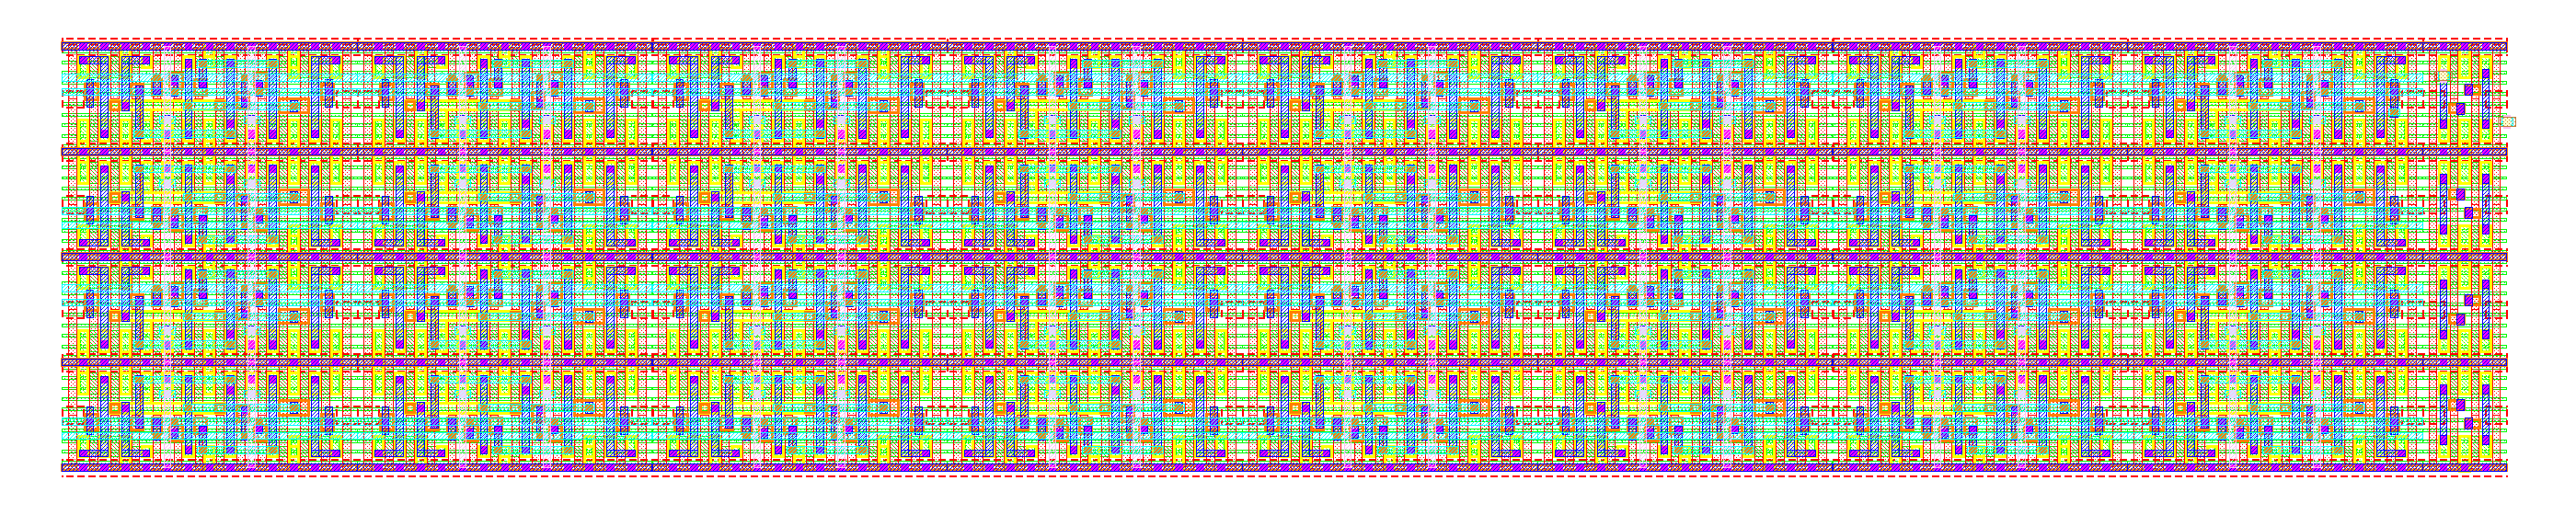
\includegraphics[width=\linewidth]{data/figures/int8x8_layout.png}
\caption{\file{b2SRAMsbc_INT8x8} layout on 2026-10-16 (routing in progress): 4 rows $\times$ 8 b2SRAMsbc, rows mirrored in pairs to share rails, one DRIVE2b at the right end of each row; $6.26 \times 1.08\,\mu\text{m}$.}
\end{figure}
\field{Decision} Row origins on multiples of 27\,nm (the 270\,nm row pitch keeps them there); bus pins only.
\field{Revisit if} the array is placed inside a larger block: its origin there must also be a multiple of 27\,nm in $y$ (and of 54\,nm in $x$).

\entry{D11. DRIVE2b: one dual-inverter drive cell per row}{2026-10-16}{d11}{Row}
\field{Question} Each row needs XB for two weights; two separate INVx1 cells (3 CPP each) sat at the row end.
\field{Options} (a) two INVx1, 6 CPP; (b) one cell, two inverters sharing their VDD / VSS source column, 4 CPP.
\field{Method} New cell \file{DRIVE2b} (schematic, symbol with A[1:0] / Z[1:0], layout from OpenLayout PCells: inverter 0 mirrored about the shared source column at $x = 108$\,nm, gates at 81 and 135\,nm, outputs Z[0] / Z[1] on M1 at 54 / 162\,nm, input contacts staggered in $y$). Each half keeps the INVx1 sizing (p2/n2, SRAM-Vt). DRC, LVS, connectivity check; DRC of a $4\times4$ block of DRIVE2b in every row mirroring and left/right flip.
\field{Result} 4 CPP $\times$ 270\,nm $= 0.058\,\mu\text{m}^2$ vs.\ $0.087$ for two INVx1 ($-33\%$, 108\,nm shorter per row). DRC clean, LVS match, and the $4\times4$ block is clean: the cell is symmetric about its source column, so any flip keeps the sources on the shared rails. With two INVx1, flipping one row's inverters left/right had put an output LISD 18\,nm from the next row's source LISD at the shared rail (LISD tip-to-tip $\ge 27$\,nm). Swapped into the array in place of the 8 INVx1 (instances x39, x49, x59, x69).
\begin{figure}[H]\centering
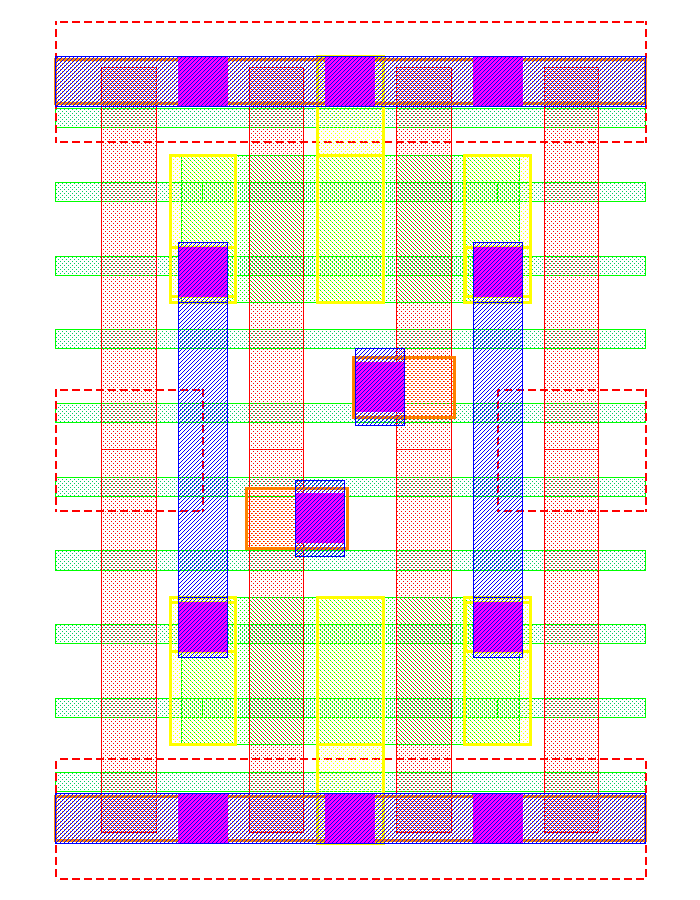
\includegraphics[width=0.32\linewidth]{data/figures/drive2b_layout.png}
\caption{DRIVE2b, 4 CPP $\times$ 270\,nm: VSS rail (bottom) and VDD rail (top), shared source column in the middle, outputs Z[0] / Z[1] on the M1 verticals at the edges, the two staggered input contacts between them.}
\end{figure}
\field{Decision} (b). XB[$i$] still drives 8 NORs: $8 \times (2 + 2) = 32$ fins from a 4-fin input, FO $\approx 8$ plus wire \verify{XB edge rate on the PEX row; D7's two-stage option if too slow}.
\field{Revisit if} the XB edge limits the cycle, or a row needs more than two inputs.

\entry{T2. Tooling notes from assembling the array}{2026-10-16}{t2}{Tooling}
Editing an OpenLayout layout in a batch script without the \file{OpenLayout_ASAP7} PCell library registered saves the transistors as static cells: LVS still passes, but the connectivity view computes terminals from default PCell parameters and reports false shorts (and chain flags such as \texttt{abut\_left} can silently change). Batch edits must register the library and change PCell parameters, not shapes. M4--M7 are SADP layers on absolute routing tracks: a minimum-width M4 wire (24\,nm) must have its lower edge at an odd multiple of 24\,nm (48\,nm pitch). Wanted next: a pin-placement tool (the array has 96 pin bits; placing them by hand is slow) and lighter KLayout highlighting while moving many instances (it loads the GPU heavily).

% =====================================================================
\section*{Open items}
\begin{itemize}
  \item Route b2SRAMsbc\_INT8x8 (D10, D11): BL/BLB down the columns, P$_k$[7:0] to the bottom edge, WL / X per row; then DRC, LVS, connectivity.
  \item Decide the reduction and accumulator: one fused carry-save tree (8 P bits per column plus the registered sum / carry fed back, one carry-propagate add at the end) vs.\ popcount, cross-column add and a ripple accumulator. Signed INT8: MSB complement plus a preloaded constant (weights); invert P and add 1 on the input's MSB cycle.
  \item Bit-exact Python reference model of the 8-weight dot product before the adder schematics.
  \item Target metric: energy per MAC (TOPS/W) at a stated throughput.
  \item SRAMCIMsbc\_INT8 still uses INVx1 (D11 replaced it in the 2-bit array).
  \item Row testbench with PEX: write a weight, toggle XB, check P[7:0]; measure P rise/fall (D5) and the XB driver (D7).
  \item Shift-accumulate adder from standard cells (16-bit, MSB-first).
  \item Corners: SS/FF models and $V_{DD}$/temperature sweeps for every delay and energy number.
  \item Hierarchical PEX results (separate session), then redo M1.
\end{itemize}

\topicindex

\end{document}
